\section{Quantitative Evaluation}\label{sec:performance}

Once the quality threshold is chosen, the key differentiator
between the speed of database construction and the quality of
reconstructed images is the hashing strategy.
We constructed 3 databases on the same set of
10,000 images sampled
from all categories of the SUN database, with image size
set to 500, and patch size set to 25, using the following
hashing strategies for Near Neighbor(NN) search:\\
\begin{enumerate}
\item \textbf{Naive NN}: 10 random projection vectors sampled from unit Normal with
uniform bin size (outliers truncated)
\item \textbf{PCA NN}: 10 first principla components as projection vectors with
bin size adapted to the distribution of projections
\item \textbf{PCA + U NN}: nearly uniform patches are hashed using Luv color
quantization into 864 bins, and non-uniform patches are handled with PCA NN
\end{enumerate}
We compare and contrast the effects of hashing on performance in
Sec.~\ref{ssec:nn-eval}, and detail a qualitative evaluation of
the results with a user study in sec.~\ref{sec:qual}.

Here we consider the quantitative performance of our system as we grow our database to 10K images.
In fig.~\ref{fig:dict_growth} we see that as for the smaller tests in sec.~\ref{sec:analysis}, the growth of our patch dictionary is sub-linear, demonstrating increasing compression benefits as more images are added to the database. We show that this trend holds for all 3 of our NN methods (\emph{naive}, \emph{pca}, and \emph{pca+u}). Note that the \emph{naive} NN approach became infeasible as the dictionary grew, as can be demonstrated by the time required to upload each successive image into the database (see fig.~\ref{fig:upload_times}). Due to this behavior, it was terminated early. We see that the two approaches using the \emph{pca} NN scheme have significantly better time performance. This is because in the \emph{naive} approach, most of the data falls in relatively few bins. Making use of \emph{pca} helps by projecting data onto the directions of maximal variance, which helps to differentiate between patches, and thus redistribute them across multiple bins. Table \ref{tab:nn-res} includes a breakdown of the number of patches and bins produced in each of the NN approaches, as well as the timings to insert images. Also, because the \emph{naive} approach has fewer bins, it is easier to find a matching patch in a bin, and thus new patches are less frequently added to the dictionary. This explains the gap we see between the red and green/blue curves in fig.~\ref{fig:dict_growth}. Another way to look at this is to consider the average number of patches added per image (see fig.~\ref{fig:ave_patches_per_img}). As more and more images are added to the database, fewer patches are added to the dictionary. We can more clearly see the gap between the red and green/blue curves in this plot. Even though we do not see the dictionary size plateauing even for our 10K image database, the trends in fig.~\ref{fig:ave_patches_per_img} are promising, and show a decline in the number of patches being added. We believe that much bigger datasets should be investigated in future work to really see the plateau effect and gain the full benefits of our patch-based compression system. Note, however, that even personal image collections are often bigger than 10K images, so this is not an unreasonable requirement.

 \begin{figure}
%\hspace{-5mm}
%\centering
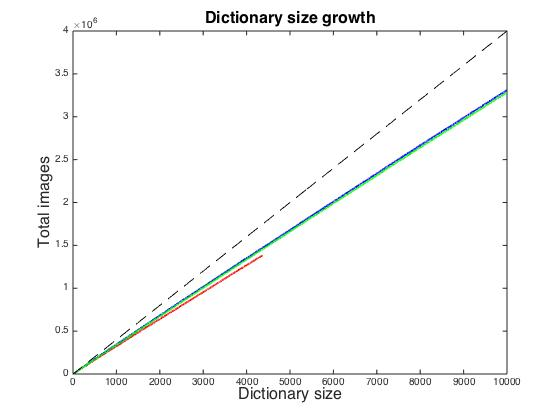
\includegraphics[width=1\linewidth]{fig_NN/dict_growth.jpg}
\caption{}
\label{fig:dict_growth}
\end{figure}

 \begin{figure}
%\hspace{-5mm}
%\centering
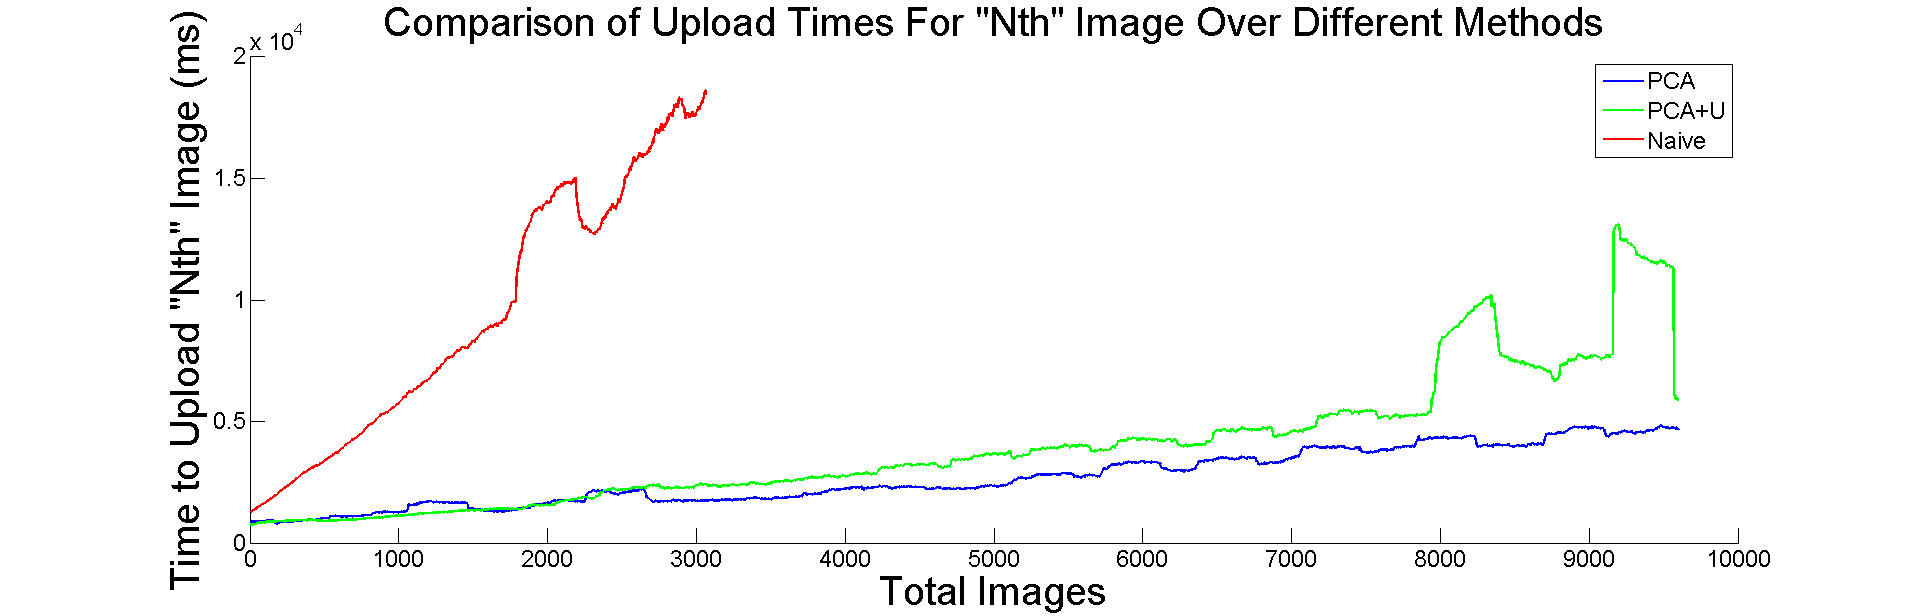
\includegraphics[width=1\linewidth]{Figures/upload_times.png}
\caption{}
\label{fig:upload_times}
\end{figure}

 \begin{figure}
%\hspace{-5mm}
%\centering
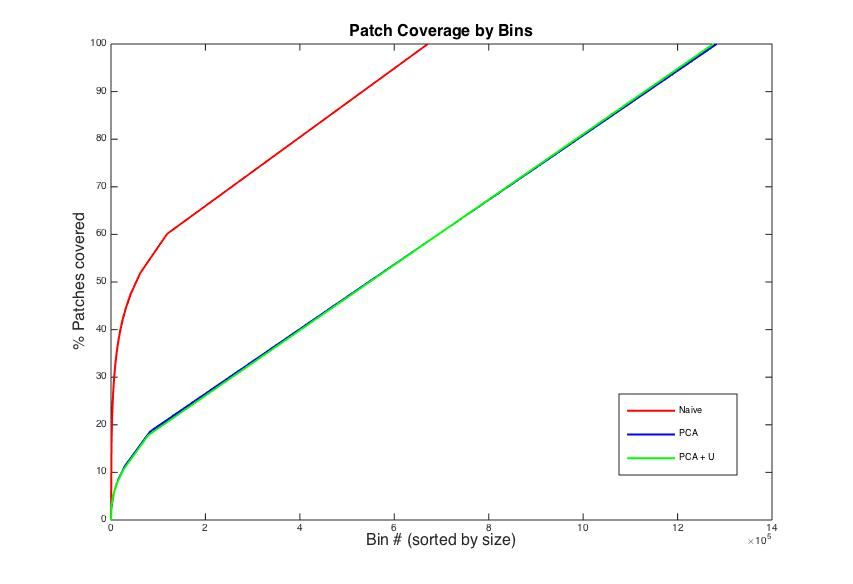
\includegraphics[width=1\linewidth]{fig_NN/bin_cover.jpg}
\caption{}
\label{fig:bin_cover}
\end{figure}

 \begin{figure}
%\hspace{-5mm}
%\centering
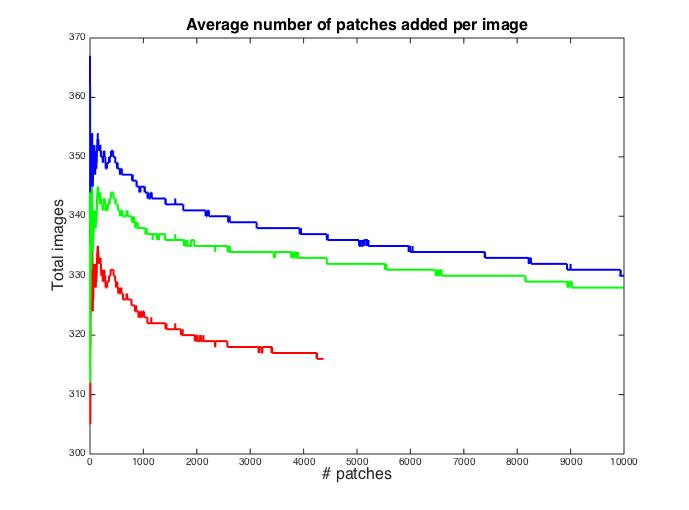
\includegraphics[width=1\linewidth]{fig_NN/ave_patches_per_img.jpg}
\caption{}
\label{fig:ave_patches_per_img}
\end{figure}

% Table
\begin{table*}
\centering
\begin{tabular}{ | c | c | c | c | c | c | c | }
\hline
& \multicolumn{3}{|c|}{Up to 4.4K} & \multicolumn{3}{|c|}{Up to 10K} \\ \hline
\textbf{method} & \textbf{time} & \textbf{\#patches} & \textbf{\#bins} & \textbf{time} & \textbf{\#patches} & \textbf{\#bins}\\
\hline
naive & 18h20min & 1,384,080 & 670,928 & n/a & n/a & n/a \\ \hline
pca & 1h54min & 1,473,592 & 1,282,768 & 7h27min & 3,309,583 & 2,751,235  \\ \hline
pca+u & 2h5min & 1,456,059 & 1,275,827 & 10h56min & 3,281,241 & 2,742,888 \\ \hline
\end{tabular}
\caption{Results on 10,000 images samples from all
the categories of the SUN database, where the rows
are for naive projection hashing, PCA-based hashing and
PCA-based hashing combine with uniform patch hashing.}
\label{tab:nn-res}
\end{table*}


\section{Qualitative Evaluation}\label{sec:qual}

For the qualitative evaluation, 3 of the paper's authors independently rated 100 randomly-selected image reconstructions from each of the three nearest neighbor methods described in sec. \ref{sec:nn}: \emph{naive}, \emph{pca}, and \emph{pca+u} (all 3 raters received the same set of images). The following rating scheme was used:

\begin{table}
\begin{tabular}{| l | l|}
 \hline
\textbf{ranking} & \textbf{requirement}  \\ \hline
5 & no visible distortions \\ \hline
4 & only minor distortions \\ \hline
3 & distortions present, but objects are recognizable  \\ \hline
2 & pretty large distortions, but scene is recognizable  \\ \hline
1 & severe distortions, scene is not recognizable  \\ \hline
\end{tabular}
\caption{The quality evaluation scheme used.}
\label{tb:rankings}
\end{table}

None of the raters received any instructions other than the rating scheme, and the evaluation was not further discussed. Nevertheless, all the raters were highly correlated with each other, where the inter-rater correlation ranged from 0.71 to 0.75 on the \emph{naive} images, 0.51 to 0.61 on the \emph{pca} images, and 0.59 to 0.64 on the \emph{pca+u} images. In figure \ref{fig:qual_method}a we plot the mean and standard error image rating for each rater and each NN method. We see some differences between the raters, but most notably, the \emph{pca} approach was rated highest across all 3 raters, and when taking the average ratings (over all 3 raters), the reconstruction quality is statistically significantly better rated for the \emph{pca} method over the \emph{naive} method. 

Next, to determine whether ratings corresponded to the actual compression ratio for the images, we correlated each of the rater's scores with the image compression ratios, and then considered different combinations of the rater scores (min, max, mean, mode, median) to see which statistic over the subjective ratings might be most predictive of the objective image compression (see table \ref{tab:corr}). Because raters are highly subjective as to what they consider a reasonable reconstruction (even given the criteria above), we will use the mean rating across all raters as it is most correlated with image compression, and most consistent. In figure \ref{fig:recon} we demonstrate the \emph{pca} NN method reconstructions of a set of images with large compression ratios, that also received high quality ratings (taking the mean across raters). This figure gives a little more insight about how our system works, because naturally, the images with the highest ratings are going to be the ones that benefit least from compression, and that is a less interesting case to consider. We are interested in reasonable reconstructions with great cost savings. We plot the trade-off between compression ratio and reconstruction quality in fig. \ref{fig:qual_method}b. As expected, quality ratings go down as the compression ratio increases. Depending on the application, the optimal point can be chosen.

\begin{table*}
\centering
\begin{tabular}{|c|c|c|c|c|c|c|c|c|}
 \hline
\textbf{method} & \textbf{rater 1} & \textbf{rater 2} & \textbf{rater 3}  & \textbf{min} & \textbf{max} & \textbf{mean} & \textbf{mode} & \textbf{median}\\ \hline
naive & 0.7337 & 0.6700 & 0.6203  & 0.7247 & 0.6837 & \textbf{0.7484} & 0.6324 & 0.6636 \\ \hline
pca & 0.7450 & 0.7916 & 0.5061 & 0.6999 & 0.6791 &  \textbf{0.8070} & 0.6695 & 0.7349 \\ \hline
pca+u & 0.6169 & 0.6685 & 0.6934 & 0.6340 & 0.6755 &  \textbf{0.7635} & 0.6043 & 0.7276  \\ \hline
\end{tabular}
\caption{Here we determine what function of rater scores is most predictive of image compression ratios. We see that the mean across the rater scores has the highest correlation with image compression, presumably because it filters out the noise inherent in subjective judgements.}
\label{tab:corr}
\end{table*}

 \begin{figure*}
%\hspace{-5mm}
%\centering
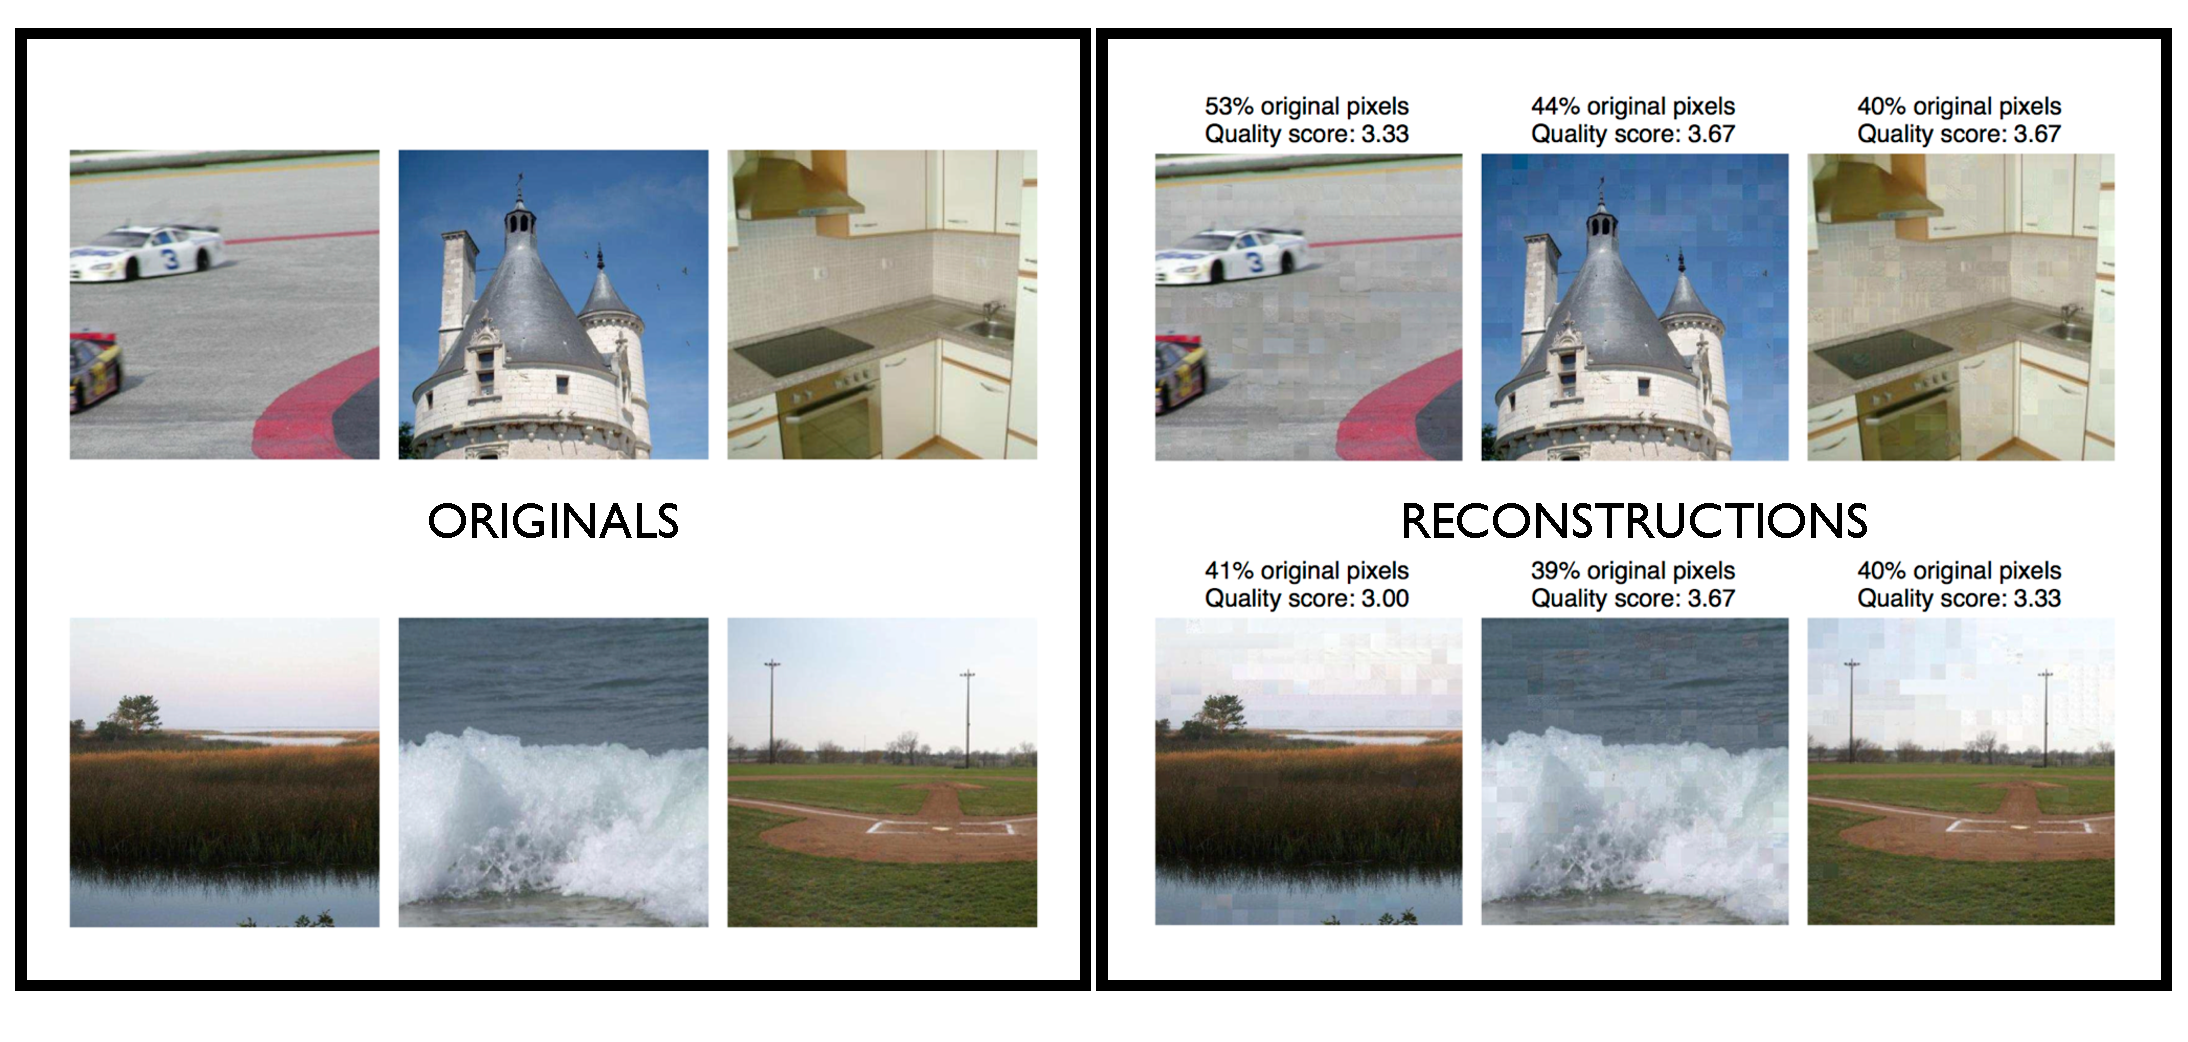
\includegraphics[width=1\linewidth]{fig_quality/orig_recon.pdf}
\caption{Here we plot 6 sample reconstructions (using the \emph{pca} NN method) that had high compression ratios \emph{and} relatively high ratings (mean over 3 raters). }
\label{fig:recon}
\end{figure*}

 \begin{figure*}
%\hspace{-5mm}
\centering
(a)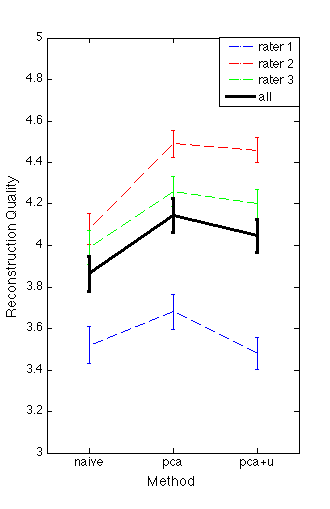
\includegraphics[width=0.3\linewidth]{fig_quality/quality_by_method.png}
(b)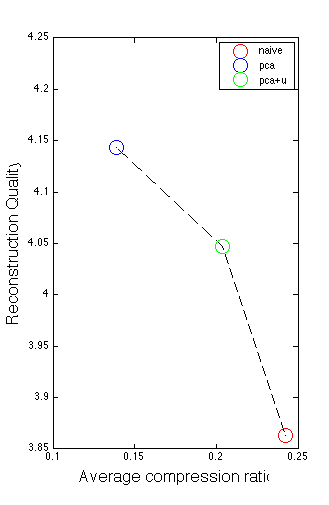
\includegraphics[width=0.3\linewidth]{fig_quality/qual_compr.png}
\caption{(a) Although there is some difference across ratings, all raters agree that the \emph{pca} NN method produces the highest quality reconstructions. (b) Reconstruction quality is inversely proportional to compression ratio. Different applications might desire different settings.}
\label{fig:qual_method}
\end{figure*}

